\documentclass{beamer}

% reduce size of title
\setbeamerfont{frametitle}{size=\normalsize}

% make a command for gray sub-items and continued subitems
\newcommand{\si}[1]{\hspace{.5cm} \textcolor{gray} {#1}\\}
\newcommand{\sicont}[1]{\hspace{1cm} \textcolor{gray} {#1}\\}

% permit absolute textblock positioning
\usepackage[absolute,overlay]{textpos}

%remove navigation symbols
\setbeamertemplate{navigation symbols}{}

\begin{document}

%% Title Page
\begin{frame}
\vspace{4cm}
\begin{center}
\normalsize{Tampa R Users Group}\\
\normalsize{06/29/2018: Group announcements}\\
\vspace{.2cm}~
\vspace{1cm}
\end{center}

\vspace{.2cm}
\begin{flushright}
\scriptsize{Travis Gerke, ScD}\\
\tiny{Organizer}\\
\tiny{travisgerke@gmail.com}\\

\includegraphics[scale=.02, trim=0 1cm 0 3.5cm, clip]{figures/Twitter_Logo_Blue.png}\tiny{\href{https://twitter.com/travisgerke}{@travisgerke}}\\
\vspace{.11cm}
\end{flushright}

\begin{textblock}{6}(0.3,12.7)
\scriptsize{
\begin{table}[h]
\centering
\begin{tabular}{l}
Meetup: \href{https://meetup.com/Tampa-R-Users-Group/}{https://meetup.com/Tampa-R-Users-Group/}\\
Web/GitHub: \href{https://tampausers.github.io/}{https://tampausers.github.io/}\\
Twitter: \href{https://twitter.com/usertampa}{@UseRTampa}\\
\end{tabular}
\end{table}
}
\end{textblock}

\begin{textblock}{6}(12,1)
\tiny{~~~~~~~~~Sponsored by:}\\

\includegraphics[width=2.2cm, trim=0 0 0 0]{figures/RConsortium_Horizontal_Pantone.png}
\end{textblock}

\begin{textblock}{6}(1,.5)

\includegraphics[width=1.5cm, trim=0 0 0 0]{figures/trug-hex-800.png}
\end{textblock}

\end{frame}

\small{

\begin{frame}[t]
\frametitle{Logo/hex sticker}
Huge shout-out to Garrick Aden-Buie for making this happen!\\
\begin{center}

\includegraphics[scale=.25, trim=0 0 0 0]{figures/trug-hex-800.png}
\end{center}
\end{frame}

\begin{frame}[t]
\frametitle{Group communication/GitHub}
A million thanks to Jordan Creed for a) running recent meetings and \\
\hspace{.5cm} b) surveying members re: communication strategies!\\
\vspace{.2cm}
Result: we are now a GitHub Organization {\tiny\href{https://github.com/TampaUseRs}{(https://github.com/TampaUseRs)}}\\
\si{Within this Org, we have a site {\tiny\href{https://tampausers.github.io/}{(https://tampausers.github.io/)}}}
\si{See instructions on landing page for joining and getting to}
\sicont{discussion/project boards}
\begin{center}
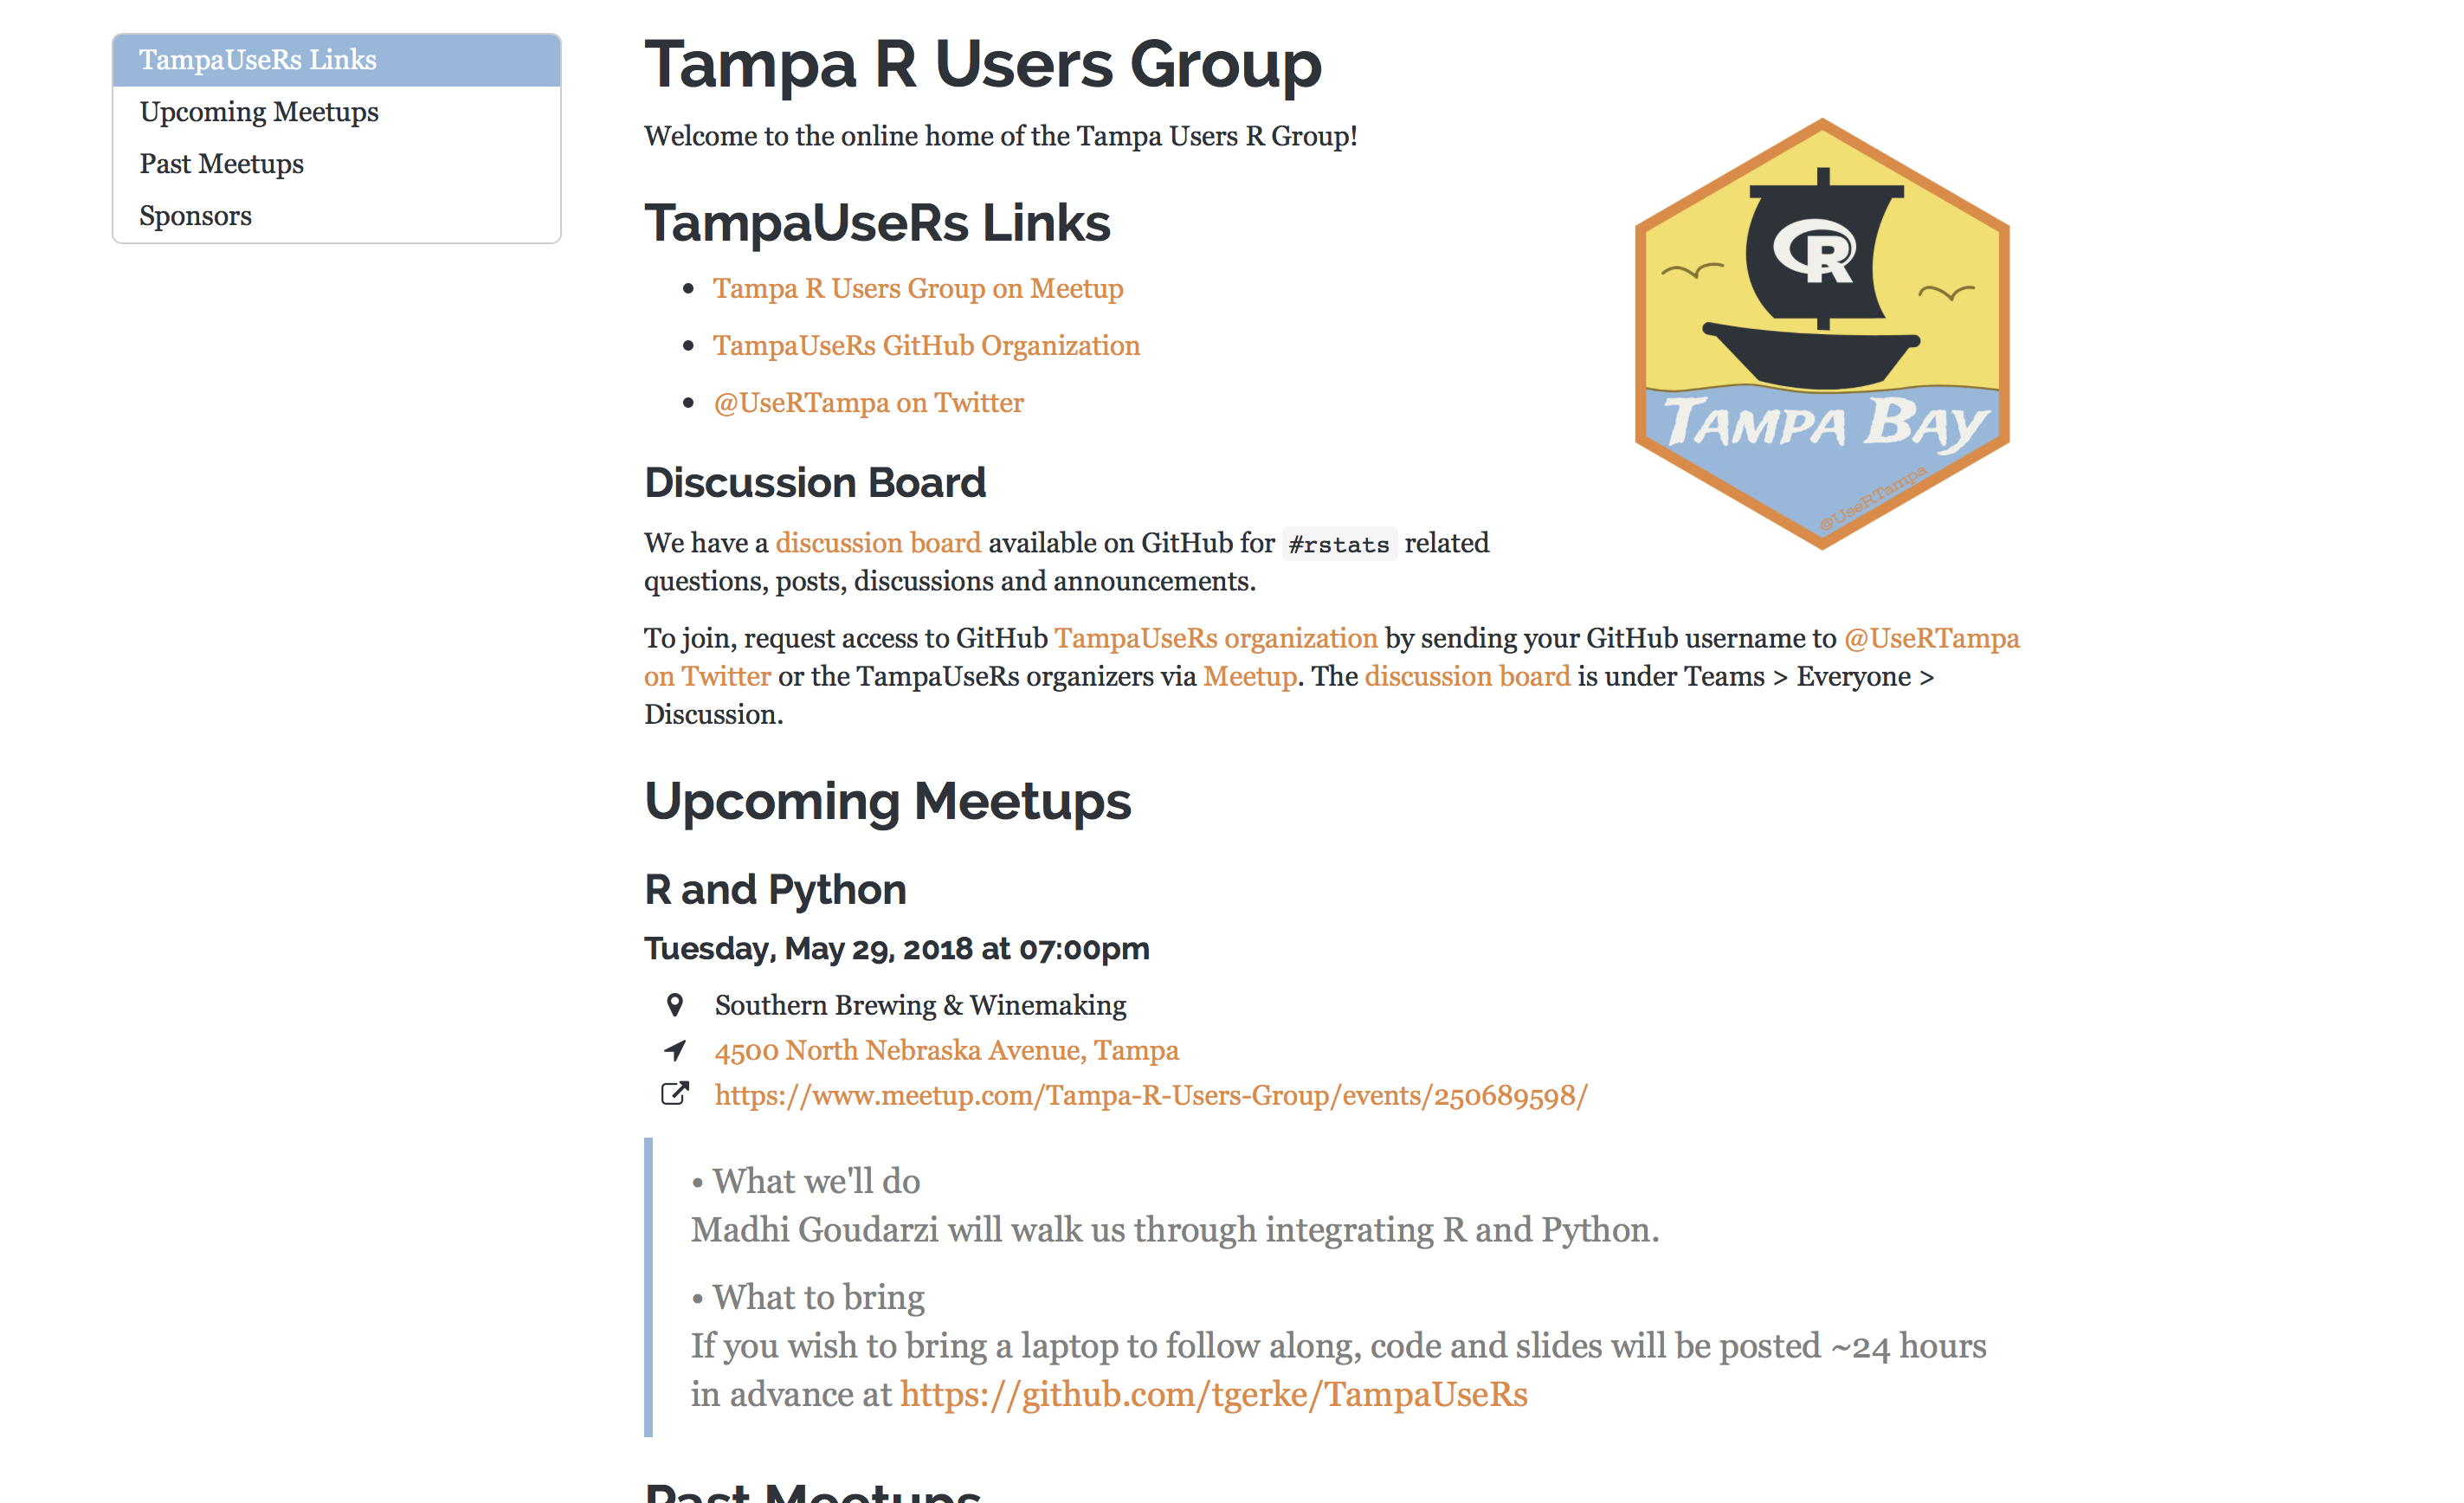
\includegraphics[scale=.25, trim=0 0 0 0]{figures/webshot.png}
\end{center}
\end{frame}

\begin{frame}[t]
\frametitle{Twitter}
Follow each other! \\
\si{DM/follow @UseRTampa for a follow from the group}
\si{We're going to put together a list of members' handles (who wish to}
\sicont{have them shared) on the GitHub page}
\vspace{.2cm}
We have grown very quickly and can have a solid network!\\
\begin{center}

\includegraphics[scale=.25, trim=0 0 0 0]{figures/members.png}
\end{center}
\end{frame}
}
\end{document}